\documentclass[a4paper,11pt,twoside,openright]{scrbook}

\usepackage{swThesis}
\usepackage{amsmath}
\usepackage{lipsum}
\usepackage{standalone}
\standalonetrue

\bibliography{bibliography}

% Figures
\graphicspath{./figs}

\begin{document}


\chapter{General Methods} \label{chapter:generalMethods}

These methods are used throughout the work in this thesis and are listed here to reduce repetition.
Each subsequent chapter will have a separate methods section which refers to methods unique to that particular chapter, 
or how they differ from the general methods described here.


\section{Cell culture}

The cell-lines were all grown in DMEM (\#21969-035 gibco) and supplemented with 10\% foetal bovine serum and 2 mM 
L-glutamine, incubated at 37$^\circ$C, humidified and 5\% CO$_2$.


\subsection{Culturing cells in 96-well plates for imaging}

Cells were seeded at roughly 3,000 cells per well (see table \ref{table:well_seeding} for cell-line specific values) 
into the inner 60 wells of a 96-well optical bottomed imaging plate (\#655090 Greiner) in 100 $\mu$L of cell culture 
media.
The outer 36 wells were filled with 100 $\mu$L PBS.
Plates were incubated for 24 hours in a tissue culture incubator before the addition of compounds.


\subsection{Culturing cells in 384-well plates for imaging}

Cells were seeded at roughly 1,500 cells per well (table \ref{table:well_seeding}) into each well of a 384-well 
optimical bottomed imaging plate (\#781091 Greiner) in 50 $\mu$L of cell culture media.
Plates were incubated for 24 hours in a tissue culture incubator before the addition of compounds.

\begin{table}[h]
\begin{footnotesize}
\begin{tabular}{@{}lll@{}}
\toprule
          & \multicolumn{2}{c}{Type of plate} \\ \midrule
Cell line & 96 well         & 384 well        \\ \midrule
HCC1569   & 3000            & 1500            \\
HCC1954   & 3000            & 1500            \\
KPL4      & 2000            & 750             \\
MCF7      & 3000            & 1500            \\
MDA-231   & 2000            & 750             \\
MDA-157   & 3500            & 2000            \\
SKBR3     & 3500            & 2000            \\
T47D      & 3000            & 1500            \\ \bottomrule
\end{tabular}
\end{footnotesize}
\captionsetup{width=0.8\textwidth}
\caption[Cell seeding densities of 96 and 384 well plates]{
    Cell seeding densities for 96 and 384 well plates.
}
\label{table:well_seeding}
\end{table}


\section{Generation of GFP labelled cell lines}

Stable GFP expressing cell lines were created from the eight breast cancer cell lines in order to aid with spheroid 
image segmentation.
Cells were seeded at approximately 35,000 cells per well of a 6-well plate in 3 mL of DMEM and incubated for 24 hours 
(37$^\circ$C) to achieve 20\% confluence.
After 24 hours of incubation, 35 $\mu$L of IncuCyte NucLight Green Lentivirus (\#4624 Essen) was added to each well at 
an  MOI of 1 with 1.5 $\mu$L of polybrene (1:2000).
Plates were then incubated for an additional 24 hours followed by a media change, and another 24 hour incubation.
Media was then changed for selection media consisting of 1 $\mu$g/mL puromycin and complete DMEM, followed by another 
24 hour incubation.
Following selection of puromycin resistant cells, cells were trypsinised and placed in a T75 tissue culture flask for 
further growth.
GFP labelled cells and parental cell-lines were compared to ensure growth characteristics remained the same.
This was achieved by measuring confluence in 6 well plates seeded with 10,000 cells per well and confluence measured 
with the Incucyte ZOOM.
Following successful transduction, GFP labelled cells were maintained in 0.5 $\mu$g/mL puromycin complete DMEM.


\section{Compound handling}

\subsection{24 compound validation set}

Compounds (table \ref{table:compounds}) were diluted in DMSO at a stock concentration of 10 mM.
Compounds plates were made in v-bottomed 96-well plates (\#3363 Corning), at 1000-fold concentration in 100\% DMSO by 
serial dilutions ranging from 10 mM to 0.3 $\mu$M in semi-log concentrations.
Compounds were added to assay plates containing cells after 24 hours of incubation by first making a 1:50 dilution in 
media to create an intermediate plate, followed by a 1:20 dilution from intermediate plate to the assay plate, with an 
overall dilution of 1:1000 from the stock compound plate to the assay plate.

\begin{table}[]
    \begin{footnotesize}
    \centering
    \captionsetup{width=0.8\textwidth}
    \caption[Annotated compounds of known MoA]{Annotated compounds and their associated mechanism-of-action label used 
in the classification tasks.}
    \label{table:compounds}
    \begin{tabular}{@{}llll@{}}
    \toprule
    Compound        & MoA class               & Supplier    & Catalog no. \\ \midrule
    Paclitaxel      & Microtubule disrupting  & Sigma       & T7402       \\
    Epothilone B    & Microtubule disrupting  & Selleckchem & S1364       \\
    Colchicine      & Microtubule disrupting  & Sigma       & C9754       \\
    Nocodazole      & Microtubule disrupting  & Sigma       & M1404       \\
    Monastrol       & Microtubule disrupting  & Sigma       & M1404       \\
    ARQ621          & Microtubule disrupting  & Selleckchem & S7355       \\
    Barasertib      & Aurora B inhibitor      & Selleckchem & S1147       \\
    ZM447439        & Aurora B inhibitor      & Selleckchem & S1103       \\
    Cytochalasin D  & Actin disrupting        & Sigma       & C8273       \\
    Cytochalasin B  & Actin disrupting        & Sigma       & C6762       \\
    Jaskplakinolide & Actin disrupting        & Tocris      & 2792        \\
    Latrunculin B   & Actin disrupting        & Sigma       & L5288       \\
    MG132           & Protein degradation     & Selleckchem & S2619       \\
    Lactacystin     & Protein degradation     & Tocris      & 2267        \\
    ALLN            & Protein degradation     & Sigma       & A6165       \\
    ALLM            & Protein degradation     & Sigma       & A6060       \\
    Emetine         & Protein synthesis       & Sigma       & E2375       \\
    Cycloheximide   & Protein synthesis       & Sigma       & 1810        \\
    Dasatinib       & Kinase inhibitor        & Selleckchem & S1021       \\
    Saracatinib     & Kinase inhibitor        & Selleckchem & S1006       \\
    Lovastatin      & Statin                  & Sigma       & PHR1285     \\
    Simvastatin     & Statin                  & Sigma       & PHR1438     \\
    Camptothecin    & DNA damaging agent      & Selleckchem & S1288       \\
    SN38            & DNA damaging agent      & Selleckchem & S4908       \\ \bottomrule
    \end{tabular}
    \end{footnotesize}
\end{table}

\paragraph{Microtubule disruptor}
The microtubule disrupting compounds (paclitaxel, epothilone B, colchine, nocodazole, monastrol, ARQ621) all act by 
disrupting tubulin.
Paclitaxel and epothilone B both stabilise microtubules by binding to the $\alpha$ and $\beta$ tubulin subunits to 
prevent depolymerisation, this over-stabilisation disrupts normal cellular functions such migration and mitosis which 
rely on the dynamic nature of the cytoskeleton.
Colchicine and Nocodazole act on the same subunits of tubulin but instead cause destabilisation of the tubulin 
structure.
Monastrol and ARQ621 are classed as microtubule disruptors but do not act on tubulin directly, instead they bind to the 
motor protein Eg5 kinesin which traverses microtubules and plays an important role in mitosis.
The microtubule disruptors typically have effects on cell-cycle and large structural changes to cell-shape.

\paragraph{Aurora B inhibitor}
Barasertib and ZM447439 bind to and inhibit Aurora B kinase, a protein involved in the spindle checkpoint during 
mitosis.
While both aurora B inhibitors and microtubule disruptors can interfere with mitosis, disrupting the spindle checkpoint 
can result in abormal cell-division and missegregation of chromosones during anaphase, whereas microtubule disruptors 
typically cause arrest of the cell-cycle.

\paragraph{Actin disrupting}
Cytochalasin D and B are actin both drugs which inhibit actin polymerisation by binding to the F-actin to stop further 
addition of actin monomers, whereas latrunculin B binds actin monomers to prevent polymerisation.
Jaskplakinolide differs in that it stabilises actin formation, although the exact mechanism is not clear.
Actin disruptors have much in common with microtubule disruptors as they both exert their effects on the cytoskeleton, 
although actin disruptors can have direct effects on apoptosis and golgi organisation.

\paragraph{Protein degradation}
MG132 and lactacystin are both proteosome inhibitors.
MG132 blocks the proteolytic activity of the 26S proteosome complex and also inhbits NF$\kappa$B activity.
Lactacystin inhibits the 20S proteosome, and also NF$\kappa$B although to a lesser extent than MG132.
ALLN and ALLM are calpain/cysteine protease inhibitors which play important roles in calcium singnalling, cell 
profileration and apoptosis.

\paragraph{Protein synthesis}
Emetine and cycloheximide both inhibit protein synthesis.
Emetine binds to the 40S ribosomal subunit, whereas cycloheximide binds to the 60S subunit.
Inhibition of protein synthesis has a wide range of effects on cellular function

\paragraph{Kinase inhibitor}
Dasatinib and saracatinib are kinase inhibitors with actions on Src kinase and Bcr-Able tyrosine kinase, although 
achieving specificity in kinase inhibitors is difficult due to conserved ATP-binding domains, so both drugs are 
reported to hit a number of other kinases.

\paragraph{Statin}
Lovastatin and simvastatin are statins, they inhibit 3-hydroxy-4-methylglutaryl-coenzyme A reductase (HMG-CoA 
reductase), a pathway responsible for the production of endogenous cholesterol.
Lovastatin and simvastatin have also been shown to inactivate RhoA which in turn can lead to apoptosis and cell-cycle 
arrest.

\paragraph{DNA damaging agent}
Camptothecin and SN38 are DNA damaging agents which act by binding and inhibiting topoisomerase I, which prevents DNA 
unwinding, causing double strand breaks and ultimately cell-death.

\begin{figure}
    \centering
    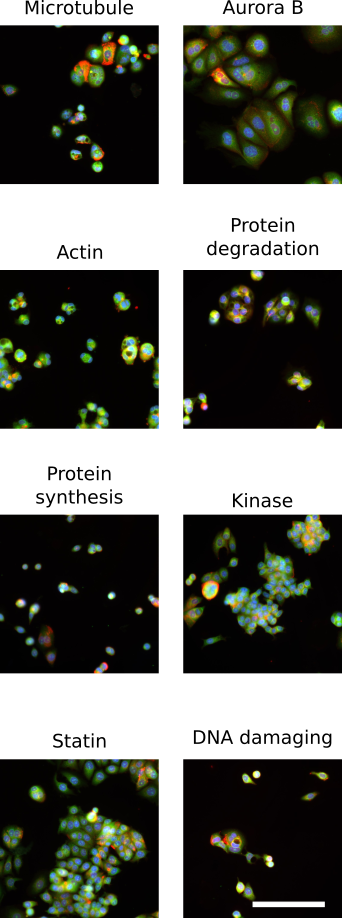
\includegraphics[width=0.5\textwidth]{ch2cellImageMOA}
    \captionsetup{width=0.8\textwidth}
    \caption[Example images of MCF7 cells for each MoA class]{
        Example images of MCF7 cells showing a typical morpholgy for each MoA class at 1 $\mu$M.
        Microtubule: paclitaxel, actin: cyctochalasin D, protein degradation: MG132, protein synthesis: emetine, kinase 
inhibitor: dasatinib, statin: lovastatin, DNA damaging: SN38.
        For untreated cells see figure \ref{figure:cell_images}.
        Channels used: Red - MitoTracker DeepRed; Green - Concanavalin A; Blue - Hoechst33342. Scale bar: 100 $\mu$m.
    }
    \label{figure:cell_images_moa}
\end{figure}


\subsection{Prestwick and BioAscent libraries}

The Prestwick approved library and 12K BioAscent libraries were screened in the same run.
Compound preparation was performed using the Biomek FX for automated liquid handling \footnote{A thankyou to Ash Makda 
(Edinburgh) for helping set up the liquid handling protocol}.
Source plates were diluted 1:10 in DMSO from 10 mM to 1 mM.
From the 1 mM compound plates 1.5 $\mu$L was transferred to an intermediate plate containing 74.5 $\mu$L of cell 
culture media for a 1:50 dilution.
From the intermediate plate 2.5 $\mu$L was transferred to the assay plate containing cells seeded in a 50 $\mu$L volume 
for a second dilution of 1:20 after factoring in estimated evaporation.
A single intermediate plate was used for 8 assay plates corresponding to the 8 cell-lines.
Assay plates were barcoded with cell-line and a sequential number corresponding to the compound source plate.
5 compound plates were screened with 8 cell-lines corresponding to 40 384-well plates each week.


\section{Cell painting staining protocol}

In order to capture a broad view of morphological changes within a cell using fluorescent microscopy, a choice has to 
be made which cellular structures to label.
This choice is limited by the availablity of the fluorescent filter sets fitted to the microscope, reagent costs, and 
the scalability of the protocol when used in a large screen.
Fortunately, this problem was already addressed by another group who published a protocol -- named ``cell painting" -- 
for labelling 7 cellular structures, using 6 non-antibody stains imaged in the same 5 fluorescent channels available 
with our miscoscopy setup. \cite{Gustafsdottir2013, Bray2016}

The cell-painting protocol was initially optimised by Gustafsdottir \textit{et al.} for use in the U2OS oesteosarcoma 
cell line, and briefly tested in a few other commonly used cell-lines.
However, when tested on the panel of 8 breast cancer cell lines, the staining protocol was observed to induce 
morphological changes on certain cell lines, in the absence of compounds.
It was found that changing the media, and adding the MitoTracker DeepRed stain to live MDA-MB-231 cells produced a 
rounded morphology, which was not observed in the other cell lines.
As any morpholgical changes introduced by the staining protocol would mask those caused by small-molecules, the 
protocol was adapted by removing the media change step, and moving the addition of wheat germ agglutinin and 
MitoTracker DeepRed until after fixation.
As the cells were now fixed immediately in their existing media this prevented any alterations to the morphology and 
improved the wheat germ agglutinin staining, although as the MitoTracker stain relies on membrane potential of the 
mitochondria, the selectivity of the MitoTracker stain was reduced when used on fixed cells, though it still produced 
selective enough labelling to capture large changes in mitochondrial morphology.

To stain cells in a 96 or 384 well plates, the cells are first fixed by adding an equal volume of 8\% paraformaldehyde 
(\#28908 Thermo Scientific) to the existing media resulting in a final paraformaldehyde concentration of 4\%, and left 
to incubate for 30 minutes at room temperature.
The plates are then washed with PBS (100 $\mu$L for a 96 well plate, 50 $\mu$L for a 384 well plate) and permeabilised 
with 0.1\% Triton-X100 solution (50 $\mu$L 96-well, 30 $\mu$L 384-well) for 20 minutes at room temperature.
A solution of cell painting reagents was made up in 1\% bovine serum albumin (BSA) solution (see table 
\ref{table:staining}).
Cell painting solution was added to plates (30 $\mu$L 96-well, 20 $\mu$L 384-well) and left to incubate for 30 minutes 
at room temperature in a dark place.
Plates were then washed with PBS (100 $\mu$L 96-well, 50 $\mu$L 384) three times, before the final aspiration plates 
were sealed with a transparent plate seal (\#PCR-SP Corning).

\begin{table}[]
    \begin{footnotesize}
    \centering
    \captionsetup{width=0.8\textwidth}
    \caption[Cell painting reagents and filter wavelengths for imaging.]{Reagents used in the cell painting protocol 
and the excitation/emission wavelengths of the filters used in imaging. ex: excitation, em: emission}
    \label{table:staining}
    \begin{tabular}{@{}lllll@{}}
    \toprule
    Stain                                                               & Labeled Structure                             
                      & \begin{tabular}[c]{@{}l@{}}Wavelength\\ (ex/em {[}nm{]})\end{tabular} & Concentration & 
\begin{tabular}[c]{@{}l@{}}Catalog no.;\\ Supplier\end{tabular} \\ \midrule
    Hoechst 33342                                                       & Nuclei                                        
                      & 387/447 $\pm 20$                                                      & 2 $\mu$g/mL   & 
\begin{tabular}[c]{@{}l@{}}\#H1399;\\ Mol. Probes\end{tabular}  \\
    Concanavalin A 488                                                  & \begin{tabular}[c]{@{}l@{}}Endoplasmic\\ 
reticulum\end{tabular}     & 462/520 $\pm 20$                                                      & 11 $\mu$/mL   & 
\begin{tabular}[c]{@{}l@{}}\#C11252;\\ Invitrogen\end{tabular}  \\
    SYTO14                                                              & Nucleoli                                      
                      & 531/593 $\pm 20$                                                      & 3 $\mu$M      & 
\begin{tabular}[c]{@{}l@{}}\#S7576;\\ Invitrogen\end{tabular}   \\
    Phalloidin 594                                                      & F-actin                                       
                      & 562/624 $\pm 20$                                                      & 0.85 U/mL     & 
\begin{tabular}[c]{@{}l@{}}\#A12381;\\ Invitrogen\end{tabular}  \\
    \begin{tabular}[c]{@{}l@{}}Wheat germ\\ agglutinin 594\end{tabular} & \begin{tabular}[c]{@{}l@{}}Golgi and \\plasma 
membrane\end{tabular} & 562/624 $\pm 20$                                                      & 8 $\mu$g/mL   & 
\begin{tabular}[c]{@{}l@{}}\#W11262;\\ Invitrogen\end{tabular}  \\
    \begin{tabular}[c]{@{}l@{}}MitoTracker\\ DeepRed\end{tabular}       & Mitochondria                                  
                      & 628/692 $\pm 20$                                                      & 0.6 $\mu$M        & 
\begin{tabular}[c]{@{}l@{}}\#M22426;\\ Invitrogen\end{tabular}  \\ \bottomrule
    \end{tabular}
    \end{footnotesize}
\end{table}


\section{Imaging}

\subsection{ImageXpress}

Imaging was carried out on an ImageXpress micro XL (MolecularDevices, USA) a multi-wavelength wide-field fluorescent 
microscope equiped with a robotic plate loader (Scara4, PAA, UK).


\subsection{Cell painting image capture}

Images were captured in 5 fluorescent channels at 20x magnification, exposure times were kept constant between plates 
and batches as to not influence intensity values.


\section{Image analysis}


\subsection{CellProfiler for 2D image analysis}

Images were analysed using CellProfiler v2.1.1 to extract morphological features.
CellProfiler \cite{Carpenter2006} was chosen primarily due to the high configurability and the permissive license 
enabling large-scale distributed processing on compute clusters in order to reduce the image analysis time.
The images captured on the ImageXpress were analysed using CellProfiler, quantifying approximately 400 morphological 
features.
The datasets produced by the CellProfiler analysis contained morphological measurements on an individual cell level, 
although this takes considerable memory requirements, and therefore single cell-level data was aggregated to image 
median profiles.
Briefly, cell nuclei were segmented in the Hoechst stained image based on intensity, clumped nuclei were separated 
based on shape.
Nuclei objects were used as seeds to detect and segment cell-bodies in the cytoplasmic stains of the additional 
channels.
Subcellular structures such as nucleoli and Golgi apparatus were segmented and assigned to parent objects (cells).
Using these masks marking the boundary of cellular objects, morphological features are measured for multiple image 
channels returning per object measurements.


\section{Data analysis}


\subsection{Preprocessing}

Out of focus and low-quality images were detected through saturation and focus measurements and removed from the 
dataset.
Image averages of single object (cell) measurements were aggregated by taking the median of each measured feature per 
image.
Feature selection was performed by calculating pair-wise correlations of features and removing one of a pair of 
features that have correlation greater than 0.9, and removing features with very low ($< 1e^{-5}$) or zero variance.
Features were standardised on a plate-by-plate basis by dividing each feature by the median DMSO response for that 
feature and scaled by a z-score ($z$) to a zero mean and unit variance by

\begin{equation} \label{eq:zscore}
    z = \frac{x - \mu}{\sigma}
\end{equation}

where $\mu$ is the mean and $\sigma$ is the standard deviation.
This is required as the measurements from CellProfiler use different scales.
For example cell area is measured in pixels and typically ranges from a few hundred to several thousand, whereas cell 
eccentricity is constrained between 0 and 1.
Large differences in feature scales causes issues with downstream pre-processing steps such as principal component 
analysis.

\paragraph{Principal component analysis}
Principal component analysis was calculated on the standardised CellProfiler features either using `prcomp` in R or 
`sklearn.decomposition.PCA' in python.
Principal components were limited to the minimum number of principal components which accounted for 80\% of the 
variance in the data.
This was calculated by obtaining the variance explained by each principal component from the PCA output as a vector 
$v$, then calculating the cumulative proportion of variance explained by successive principal components as the 
cumulative sum of $v$ divided element-wise by the sum of $v$ to yield a new vector $w$ of the same length.
Then by finding the minimum index of $w$ at which the value of $w_i \geq p$ (where $p$ is the portion of variance to be 
explained) returns the number $n$, where principal components $[1, \dots, n]$ where used as a features.

\end{document}
